\documentclass[12pt, titlepage, a4paper]{article}
\usepackage[utf8]{inputenc}
\usepackage{changepage}
\usepackage{prftree}
\usepackage{amssymb}
\usepackage{amsmath}
\usepackage{enumitem} 
\usepackage{graphicx}
\usepackage{wrapfig}
\usepackage[spanish]{babel}
\usepackage{amsthm}
\usepackage{bussproofs}
\usepackage{bm}
\usepackage{url}
\usepackage{hyperref}
\usepackage{dirtytalk}
\usepackage{algorithm}
\usepackage{algorithmic}
\usepackage{float}


\usepackage{titlesec}
\usepackage[export]{adjustbox}

\usepackage{indentfirst}

\setcounter{secnumdepth}{4}

\titleformat{\paragraph}
{\normalfont\normalsize\bfseries}{\theparagraph}{1em}{}
\titlespacing*{\paragraph}
{0pt}{3.25ex plus 1ex minus .2ex}{1.5ex plus .2ex}

\usepackage[a4paper, total={6in, 8in}]{geometry}


\title{Trabajo PRactico Final\\ Inteligencia Artificial}
\author{Agustin Fernandez Berge y Ramiro Gatto}

\begin{document}
\maketitle

\section{Introducción}
La idea principal del proyecto es usar InceptionV3 para poder clasificar los distintos \say{sellos} (gestos con las manos) del anime de Naruto. Ademas, también realizar fine-tuning sobre las ultimas capas para mejorar el modelo.\\

\begin{figure}[h]
    \centering
    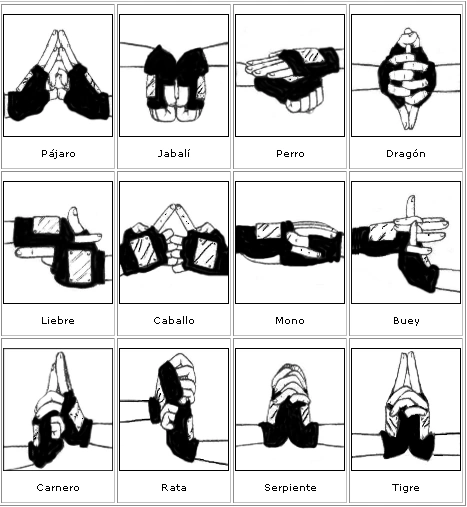
\includegraphics[width=0.5\textwidth]{Imagenes/Sellos_Basicos.png}
    \caption{Sellos Basicos}
\end{figure}

Para el proyecto se utilizaron 3 dataset de proyectos similar (primero empezamos con uno y lo fuimos ampliando), mas una cuantas imágenes que agregamos para que este sea un poco mas variado.\\


\section{Primeros pasos}
\subsection{Primer Problema}
Lo primero que hicimos fue leer el materia subido en la pagina de keras sobre InceptionV3 con fine-tuning \cite{Paginakeras}
Usando este primer modelo mas un poco de información extra para poder adaptarlo a mas de 2 clases (el ejemplo de keras solo tiene dos clases) llegamos a un modelo que posee el siguiente accuracy:

\begin{itemize}
    \item Accuracy Train: Superior al 80\%
    \item Accuracy Validation: Entorno al 50\%
    \item Accuracy Test: Entorno al 20\%
\end{itemize}

Donde claramente se ve que ocurre (muy notablemente) overfitting. Ademas, cuando lo queríamos probar para ver si al menos clasificaba bien los ejemplos del train este los clasificaba casi siempre mal.\\

\subsection{Primera Solución}
Entonces como primer medida pensamos que el modelo podría clasificar mal las imágenes debido a que estas eran muy poco \say{claras}, debido a que eran de poca resolución y las manos eran un poco \say{particulares}. Sumándole el hecho de que hay algunos \say{sellos} muy parecidos, llegamos a una primera conclusion de que estos factores hacían que el modelo no aprendiese bien.

Entonces como primera solución que aplicamos fue ampliar el dataset, con otros dataset, con manos diferentes al que teníamos, mas el agregado de imágenes que sacamos de este canal de youtube \cite{CanalOtaku}
el cual hace lo gestos con diferentes atuendos, dándonos el agregado de variedad que necesitábamos.\\

\section{Continúan los problemas}
\subsection{Continua el problema}
A pesar de haber agregado mas ejemplos y que haya mas variedad seguiamos teniendo overfitting. Era mucho menor teniendo los siguiente resultados para el train y test:

\begin{itemize}
    \item Accuracy Train: Entorno al 90%
    \item Accuracy Test: Entorno al 60%
\end{itemize}

Ademas seguíamos teniendo el problema de que al probar con ejemplos del train, que deberían dar casi siempre bien por el alto accuracy, las clasificaba mal.

\subsection{Segunda solución}
Pensamos y aplicamos muchas soluciones, esta por separado no fueron muy útiles (mejoraban ligeramente) pero fue cuando las combinamos que se noto un poco mas la mejora; estas fueron:
\begin{itemize}
    \item Como primer medida pensamos que el learning rate ($\alpha$) no era demasiado chico (al crear el modelo y en el fine-tunning). Entonces lo redujimos en ambos casos, haciendo que el del fine-tunning sea menor y que se pueda achicar si es necesario al momento de entrenar.
    \item La subsecuente medida que se nos ocurrió fue cambiar el fine-tunning. Ahora en vez de congelar y descongelar la ultima capa, lo hacemos con mas (probamos primero con 50 y luego con 100, quedándonos con las 100)
    \item También, pensamos que los ejemplos actuales podían no ser suficientes, asi que agregamos data aumentation para mitgar esto (ya no encontramos mas datasets)
\end{itemize}

\section{Un nuevo problema}
\subsection{Nada es lo que parece}
Con los cambios que explicamos en la sección anterior hubo una mejora en cuanto a los resultados. Ya el overfitting era mucho menos, la diferencia entre los accuracy del train y test era del solo del 10\% en casi todos los casos.

Pero seguíamos teniendo el problema de que clasificaba prácticamente siempre todas las imágenes. En este punto no entendíamos bien los que pasaba al hacer el test/train saca un accuracy alto (en ambos caso era mayor de 70\%) pero al probarlo nosotros siempre calificaba mal (con estos numero al probar 5 imágenes random debería clasificar al menos 3 bien pero nunca pasaba esto, casi siempre clasificaba mal las 5).

\subsection{Busqueda del problema}
En un inicio lo que pensamos es que el modelo confundía \say{sellos} que serian parecidos (como puede ser \say{rat}, \say{ram}, \say{tiger} o \say{snake}, \say{boar}).\\

Asi que lo que hicimos fue rehacer el modelo pero juntando las clases parecidas. De esta forma podríamos saber si en efecto las confunde o el problema es por otra coso.\\

Para nuestra desgracia el problema no era por ahi, al juntar las clases parecidas el modelo anda mucho mejor. Es decir con valores altos de los accuracies y no fallando al probarlo con ejemplos del dataset y con ejemplos por fuera de este.\\

Una solución que nos dieron fue ver las permutaciones de los 12 \say{sellos} en grupos de 3, ver cuales se podían juntar y por cada conjunto crear un modelo y a esto sumarle un modelo para poder ver a que grupo pertenecia. Asi el ultimo modelo me dice a que modelo debo mandar la imagen para que el siguiente modelo lo clasifique (esto fue lo que entendimos). Tratamos de ver si esto era posible, sacando las cuneta tendríamos que probar permutaciones de 3 clases de las 12 posibles. Si cada modelo tarda 30 minutos en hacerce tardariamos casi 40000 minutos o mas de 1500 días para obtener todos los posibles modelos (algo que es casi imposible de lograr en esta vida), asi que tratamos de buscar otra solución.

\subsection{Solución que aplicamos}
Viendo que la solucion anterior era practicamente imposible de realizar deicidmo ver que otro parametro podriamos modificar para que el problema desaparezca.\\

Entonces realizamos los siguientes cambios:
\begin{itemize}
    \item Cuando realizábamos el $model.compile$ ulizabamos $CategoricalCrossentropy()$ para el $loss$, ahora realizamos $CategoricalFocalCrossentropy()$. Debido a que este ultimo .... (COMPLETAR).
    \item Una cosa que sacamos fue le dropout al momento de crear el modelo. Si bien la idea del dropout es perturbar el modelo en cada iteración de entrenamiento para que puede aprender de otras formas los conceptos, vimos que en nuestro caso es contraproducente porque ... (COMPLETAR)
    \item También agregamos la función de que corte el entrenamiento luego de cierto tiempo. Si bien usamos el $StopErlay$ para que corte ante si no hay una mejora, a veces esta mejora era muy ínfima y hacia que el modelo tarde mucho. \\
    Al cortarlo antes nos aramos tener que esperar de mas por una mejora del menos del 1\% en los accuracy.\\
    Esto fue mas que nada para poder probar un poco mas de vece y evitar que la computadora se muera en el proceso.
\end{itemize}

Luego de realizar estos cambios el modelo tenia un accuracy de train mayor al 90\% y un accuracy de train mayor al 80\%, y ahora al probarlo clasificaba bien los ejemplo cuando los probábamos nosotros.

\newpage

\bibliographystyle{unsrt}
\bibliography{lib}


\end{document}